\documentclass{listhesis}
% --- Listhesis builds on KOMA script report (scrreprt).
%     Class arguments are passed to that class.

% --- Add additional packages here using \usepackage{package-name}.

% --- Provide your thesis details here.
\setup{%
  % de,                   % uncomment if your thesis is in German
  author=Iffat Brekhna, % your name
  title={Simulator Support for Dynamic Data Migration},
  date={May 21, 2018}, % submission date (today is used if unset)
  type=master,        % thesis type [master, bachelor, research, internship, diplom]
  advisor=Sven Rheindt M.Sc, % your advisor (typically some PhD. student)
  supervisor=Prof. Dr. sc. techn. Andreas Herkersdorf, % your supervisor
  % % uncomment the next lines if your thesis was carried out in industry
  % company=External Company,
  % externalAdvisor=Your Companyadvisor
}

\begin{document}

\maketitle
\cleardoublepage

% --- Thesis abstract.
%     For German thesis also provide an English version via the optional
%     argument: \anstract[English]{German}
\abstract{An abstract is defined as an abbreviated accurate
  representation of the contents of a document. -- American National
  Standards Institute (ANSI)}
\makeabstract
\clearpage

% --- Content tables.
\tableofcontents
\clearpage
\listoffigures
\clearpage
\listoftables
\clearpage

% --- Your thesis starts here.
%     Use \chapter{}, \section{}, \subsection{}, \subsubsection{},
%     and \paragraph{} to structure your thesis.

\chapter{Introduction}
\section{Motivation}
Current research in semi-conductor industry is towards developing a single chip multi-tile multi-core processor. Hence, parallel programming is experiencing a rapid growth with the advent of such system on chip (SoC) architectures. One example of such a processor is the Invasic architecture~\cite{invasive} as shown in Figure \ref{fig:multi-core,tile}. The main idea of this architecture is to introduce ``resource aware programming" support so that a program has the ability to explore its surroundings and dynamically spread its computations to neighboring processors~\cite{invasive}. Because of multiple tiles and cores on one chip these processors deal with data processing at a high scale and complexity. Therefore, the bottleneck have shifted from computational complexities to data management capacities.\\
\\
Since modern, scalable multiprocessor system-on-chip (MPSoC) platforms have Non-Uniform Memory Access (NUMA) properties, application performance is highly influenced by data-to-task locality. The goal is to bring tasks and data closer together to increase overall performance. This is a twofold and complementary problem consisting of data and or task migration. In this thesis, we will look into data placement and see how it improves the performance of the MPSoC.\\
\\
We propose a dynamic data migration (DDM) scheme in which the data is migrated dynamically at run time from one Tile Local Memory (TLM) to another TLM if the need arises. This is the major differentiating factor of our approach, managing data placement at run time rather than at compile time.
\section{Problem}
The research in the group is given in~\cite{lispaper}. They describes how the data is placed on the local memory. The data used by an application is divided at the granularity of cache lines and migrated from the global memory to the local memory according to the ideal location that is derived based on the task-to-data mapping techniques. They propose two techniques on how to do this task-to-data mapping; First Touch Policy and Most Accesses Policy. As the names suggest in first touch the memory blocks are migrated to the TLM of the tile that accesses the data first whereas in most accessed the memory blocks are migrated to the TLM of the tile that accesses it the most over the complete application~\cite{lispaper}. \\
\\
The drawback of the most access policy is that the evaluation is performed for a complete application's runtime so data cannot be migrated dynamically at run time but instead it is only migrated statically at compile time. Also in both the policies (most access policy and first touch policy) once the data is placed on TLM's that placement is fixed, you cannot change it even if the placement is having negative effects on the performance of the processor. You have to restart the application  to run the algorithm again if you want to change the data placement. 
\begin{figure}[h!]
  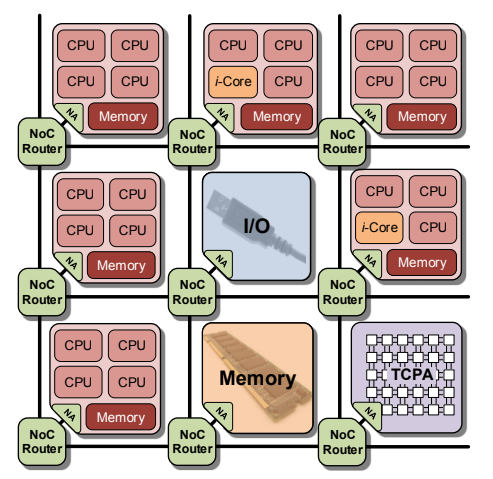
\includegraphics[width=0.7\linewidth]{multi-core,tile.png}
  \centering
  \caption{Invasic Architecture~\cite{iNetworkAdapter}}
  \label{fig:multi-core,tile}
\end{figure}
\section{Goals of Thesis}
The goal of this thesis is to design, implement and evaluate a dynamic data migration technique for memory management at run time. The system will evaluate itself and find the best data placement to improve it's performance. \\
\\
The outcome will be a system which does not need external support to find the best placement for its memory but rather it will adapt itself to place the data at the best location which will in turn improve the performance. 
\section{Approach}
The steps followed to develop the Simulator Support for Dynamic Data Migration are as follows:
\begin{itemize}
  \item Understanding the Idea: In this step, the purpose is to understand why we need data migration in the first place and how data placement is done on a distributed shared memory before the application runs. We look into other means of bringing the data close to the processor as well. 
  \item Literature Review: Find and read relevant work that has already been done for bringing the data and process/task together. Choose one approach on how to bring data and task together and find relevant ideas to understanding the concept better. 
  \item Design: Here we decide which technologies to use and how to design our system for optimal results. We want a design thats easy to change, extend, optimize and is scalable. Also, we decide how we will evaluate our system eventually and what metrics we will use in result gathering. 
  \item Implementation: Implement the design of the solution. 
  \item Evaluation and Testing: Compare the results of thesis with static data placement results. --complete this after you get results iffat
  \item Writing Report: Compose a document that explains the system in detail and depict the results obtained from using this system.
\end{itemize}
\section{Outline}
The work is structured as follows. In Chapter 1 a brief introduction of the problem is given along with the motivation to solve it and then a brief overview of the solution is given.
In Chapter 2 the basic concepts needed to understand how dynamic data migration is implemented are explained along with the work already done related to this thesis is given. In Chapter 3 the system architecture is introduced i.e the modules added for implementing dynamic data migration are introduced and explained. In Chapter 4 the implementation is explained in detail. In Chapter 5 the the programs that assisted or were used for running the simulations before gathering results are given. In Chapter 6 the results are presented. It shows how the performance has changed with the proposed solution implementation.In Chapter 7 a summary is given and some suggestions for future works in this domain. 
\chapter{Background and Related Work}
In this chapter the necessary background information is introduced in order to understand the thesis. Moreover, we will discuss the related work in this domain of research.\\
\\
\section{Basic Concepts}
\subsection{Tile}
Figure \ref{fig:tile} shows a single tile. You can see in the figure that it composes of four CPU cores, L1 caches for every core, L2 cache which is shared between all the cores and a Tile Local Memory (TLM) which is also shared by all the cores. It also has a Bus which connects the cores to the L2 Cache and the TLM. Each component of the tile is explained below.\\
\par
\textbf{Core}: A CPU Core is the basic processing unit that receives instructions(from the user or application) and performs calculations based on those instructions. A processor can have a single core or multiple cores. \\ 
\par
\textbf{TLM}: TLM stands for Tile Local Memory. Each tile has its own TLM which is shared among all the cores of the tile~\cite{ankitThesis},~\cite{iNetworkAdapter}. This memory is cachable by the L1 caches of all the cores in the tile it sits on and by the L2 cache of any other tile. The TLM from one tile can be accessed by the core of another tile.\\
\par
\textbf{Bus}: The bus connects the cores to the L2 Cache and the TLM and to other tiles. When accessing another tile the request has to go through a network adapter to be routed to the destination tile. We are using a ...Iffat ask about this!!\\
\par
\textbf{Network Adapter (NA)}: The network adapter provides the interface between a tile and the network connection which is providing a connection to other tiles and the DDR.\\
\par
\textbf{Cache}: Cache is a temporary storage space which is made up of high-speed static RAM (sRAM). It stores information which has been recently accessed so that it can be quickly accessed at a later time. It operates on the principle that most programs access information or data over and over again so by having data in the SRAM the CPU does not access the slow DRAM again and again. A cache hit occurs when the processor core accesses data that is already present in the cache whereas a cache miss occurs when the data is not present in the cache and has to be fetched from the TLM or the main memory to the cache. In our architecture we have two levels of caches:
\begin{itemize}
  \item L1 Cache: Level 1 cache (L1 Cache) is the cache right next to the core and is the smallest in size. It is not shared with any other core i.e it is a private cache.
  \item L2 Cache:Level 2 cache (L2 Cache) is away from the processor and is larger in size than the L1 cache. It is shared between all the cores in a tile. In our scenario, L2 cache is the Last Level Cache (LLC) in the system.
\end{itemize}
\begin{figure}
  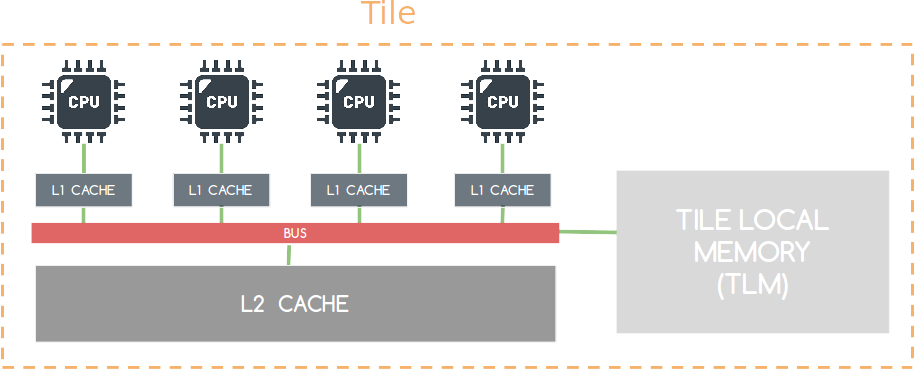
\includegraphics[width=\linewidth]{tile.png}
  \centering
  \caption{A Tile}
  \label{fig:tile}
\end{figure}
\section{Related Work}
The main idea is to bring data and tasks close together in order to save execution time used in transferring data back and forth and increase overall performance. This can be done in several ways e.g by placing and migrating data in the cache, in the local memory or by migrating tasks to the data instead. These different ideas on how it has been done are discussed in the subsections below. 
\subsection{Data Placement/Migration on Caches}
This section explicitly talks about how data placement and migration has been implemented in caches. 
A great amount of work have been done on data-placement in the shared last level cache in order to reduce the distance of data from the core requesting the data and to take care of load balancing across the chip.\\
\\
In static data placement~\cite{cacheDataPlacement1},~\cite{cacheDataPlacement2} the whole address space is divided into subsets and every subset is mapped to a LLC slice regardless of the location of the requesting core which leads to unnecessary on-chip traffic. Its advantage is that it evenly distributes the data among the available LLC slices and reduces off-chip accesses. In dynamic data placement~\cite{cacheDataPlacement1},~\cite{cacheDataPlacement3},~\cite{cacheDataPlacement4} the data blocks are placed such as to reduce the distance between the data block's home node and the core requesting it. This eliminates the unnecessary on-chip traffic. It requires a lookup mechanism to locate the dynamically selected home node for each data block. In reactive data placement data is classified as private or shared using the operating systems page tables at page granularity~\cite{cacheDataPlacement4},~\cite{cacheDataPlacement6}. Because all placement is performed at page granularity level there is load imbalance as some LLC slices might have higher accesses compared to others. This load imbalance leads to hot-spots~\cite{cacheDataPlacement6}.\\
\\
There is a hybrid data placement~\cite{cacheDataPlacement6} which combines the best features of static and dynamic data placement techniques. It optimizes data locality and also takes care of load balancing of the shared data. Hybrid data placement differs from Reactive data placement in regard to allocation of shared data among the cores i.e in Hybrid data placement, data is also classified as private or shared using the operating systems page tables but when a page is classified as shared (in hybrid data placement) it is allocated to a cluster of LLC slices and within this cluster the page is statically interleaved at the granularity of cache lines~\cite{cacheDataPlacement6}. This balances the load among the LLC slices.\\
\subsection{Task/Thread Placement}
Placing threads that share data on the same core improves performance~\cite{threadPlacement1}. However, finding the optimal mapping between threads and cores is a NP-hard problem~\cite{threadPlacement2} and cannot be scaled. One way to solve this problem is by monitoring the data accesses to determine the interaction between threads and the demands on cache memory~\cite{threadPlacement3}. In~\cite{threadPlacement3} a mechanism is there to transform the number of memory accesses from different threads to communication patterns and use these patterns to place the threads that share data on cores that share levels of cache.  They generate a communication matrix using the number of accesses to the same memory location by two threads and then maps the threads with highest communication to the same core. The disadvantage of this method is that generating the communication matrix through simulation is slow and they propose the application vendor provides this matrix with the application.\\
\\
In~\cite{threadPlacement4} a thread scheduling mechanism is proposed which uses the performance monitoring unit (PMU) with integrated hardware performance counters (HPCs) available in today's processors to automatically re-cluster threads online. Using HPSs they monitor the stall breakdowns to check if cross chip communication is the reason for the stalls. If that is so, they detect the sharing pattern between the threads using the data sampling feature of the PMU.  For every thread they maintain a summary vector called the shMap  which holds the signature of data regions accessed by the thread which resulted in cross-chip communication. These shMaps are analyzed i.e threads with high degree of sharing will have similar shMaps and will be placed to the same cluster. The OS then migrates the threads with higher sharing to the same cluster and place them as close as possible~\cite{threadPlacement4}.\\
\subsection{Data and Thread Migration}
In~\cite{datathreadPlacement} a mechanism called CDCS is presented which using a combination of hardware and software techniques jointly places threads and data in multi-cores with distributed shared caches. CDCS takes a multi-step approach to solve the various interdependencies. It places data first and then places threads such that the threads are close to the center of mass of their data. Then using the thread placement it again re-place the data and once again for this data it re-places the threads to get a optimum placement. This technique improves performance and energy efficiency for both thread clustering and NUCA techniques~\cite{datathreadPlacement}.\\
\subsection{Data Placement on TLM}
This section talks about the data placement mechanisms on the tile local memory.
\subsubsection{Static Data Placement on TLM}
In~\cite{lispaper} the authors have implemented static data placement for the tile local memory. They divide the data used by an application at the granularity of cache lines and migrate it from the global memory to the local memory according to a ideal location that is derived based on the task-to-data mapping techniques. They propose two schemes on how to do this task-to-data mapping:
\par
\textbf{First Touch Policy}: As the names suggest in First Touch Policy the memory blocks are migrated to the TLM of the tile that accesses the data first. 
\par
\textbf{Most Accesses Policy}: In Most Accessed Policy the memory blocks are migrated to the TLM of the tile that accesses it the most over the complete application runtime. The drawback of this policy is that the evaluation is performed for a complete application's runtime so data cannot be migrated dynamically at run time but instead it is only migrated statically at compile time.
\subsubsection{Dynamic Data Placement and Migration on TLM}
In~\cite{dynamicPageMigration} the authors have proposed a dynamic page migration scheme for a multiprocessor architecture using a mesh connection with a distributed global memory as shown in figure \ref{fig:mesh} . They use the \textit{pivot} mechanism to regulate the dynamic migration of pages by keeping track of the access pattern to every local page in every distributed memory module. If the access pattern is unbalanced then the page pivots to the nearest neighbor in the direction which caused the unbalanced access pattern.\\
\\
In acquiring the results the authors assumed two sets of conditions:
\begin{itemize}
	\item infinite memory space model i.e it is assumed that the destination memory module always has free space
	\item finite memory space model i.e a page is only allowed to migrate if its destination memory module has free space
\end{itemize}
The authors collected their results by seeing how the dynamic page migration scheme improved their number of hops. In all the cases the hops were reduced, but the effect is more dominant when the pivot factor (threshold value) is small.\\
\begin{figure}
  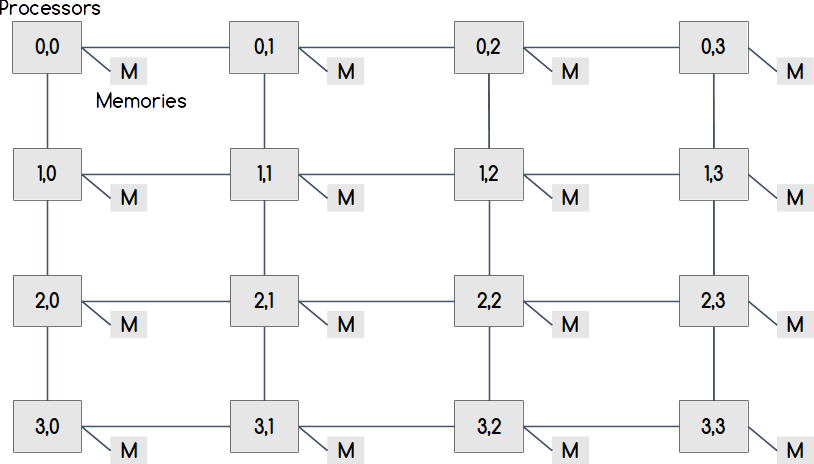
\includegraphics[width=0.7\linewidth]{meshconnected.png}
  \centering
  \caption{A mesh-connected distributed global memory system with 16 processors~\cite{dynamicPageMigration}.}
  \label{fig:mesh}
\end{figure}
\chapter{System Architecture and Concept}
This chapter will talk about the technologies used to develop the system and will illustrate and explain the architecture and design of the system. It will further explain each module in detail.
\section{Tools and Technologies}
The simulator is created in Synopsys Platform Architect MCO. Synopsys Platform Architect is a SystemC TLM standards-based graphical environment for capturing, configuring, simulating, and analyzing the system-level performance and power of multi-core systems and next generation SoC architectures~\cite{synopsys}.
The system was programmed in SystemC TLM-2.0 as it is a system-level modeling language. It provides communication-oriented, event-driven simulation interference. TLM is transaction-level modeling in which the details of communication among modules are separated from the details of the implementation of the functional modules~\cite{tlm}. TLM-2.0 focuses on memory mapped bus modeling which is fast and accurate.
\section{Concept}
In~\cite{dynamicPageMigration}, the authors have implemented a dynamic page migration scheme for a multiprocessor architecture which has mesh connection with a distributed global memory as shown in figure \ref{fig:mesh}. We differ from their scheme as they have done migration at the granularity of pages whereas we want to do it at the granularity of a TLM Block which can vary in size from one cache line to multiple cache lines. Also, our architecture differs from theirs as we have tiles (not processors) connected in a Network on Chip (NoC) as shown in figure \ref{fig:processor}.\\
\\
In ~\cite{cacheDataPlacement1},~\cite{cacheDataPlacement3} and~\cite{cacheDataPlacement4} the authors have done dynamic data placement for the last level cache (LLC) in order to reduce the distance between the data blocks and the core requesting it. We also want to bring data and the core requesting the data close together but we dynamically migrate the distributed shared tile local memory (TLM) instead of the LLC. For that we need to monitor the accesses made to the TLM of every tile in order to decide if migration is needed or not. The individual modules used in implementing this scheme will be explained in detail in the next chapter.\\
\begin{figure}
  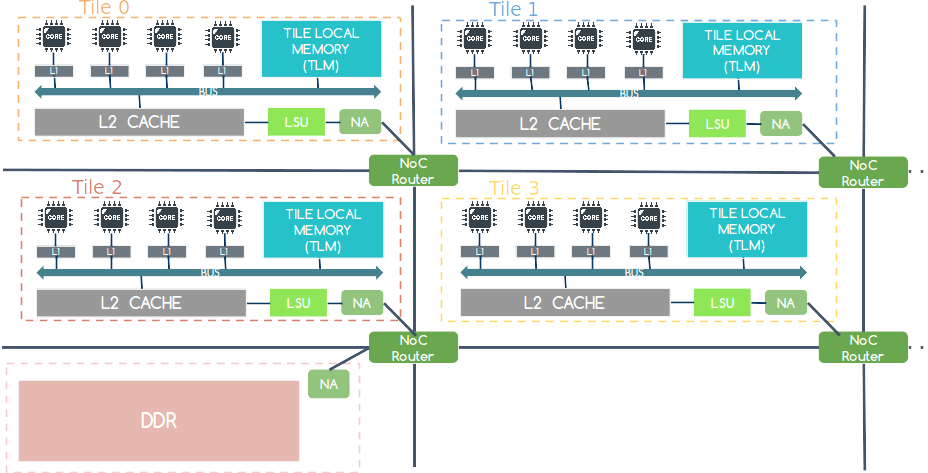
\includegraphics[width=\linewidth]{processor.png}
  \centering
  \caption{Our architecture.}
  \label{fig:processor}
\end{figure}
\chapter{Implementation}
In this chapter the detailed approach of the system and the design used to develop the simulator have been discussed. The individual modules are also explained. We further talk in detail about what how the parameters responsible for data migration are calculated and the limitations that exists in the simulator. 
\section{Tile Local Memory}
The Tile Local Memory (TLM) is a distributed-shared memory in the processor architecture. By distributed-shared we mean that it is distributed among all the tiles and can be accessed by core's placed remotely on neighboring or far away tiles. 
\subsection{Types of Accesses to TLM}
As mentioned in the previous chapter, figure \ref{fig:tile} depicts the inside of one tile. We have multiple such tiles in our processor hence the name multi-tile multi-core processor architecture.
\subsubsection{Local TLM Accesses}
Figure \ref{fig:localaccesses} depicts a scenario where a core is accessing its own tile's TLM which makes it a local TLM access. In this scenario the data transfer is happening just inside the tile and there is no traffic going outside the tile to the bus. This takes less time as data is placed close to the core that uses it. 
\begin{figure}
  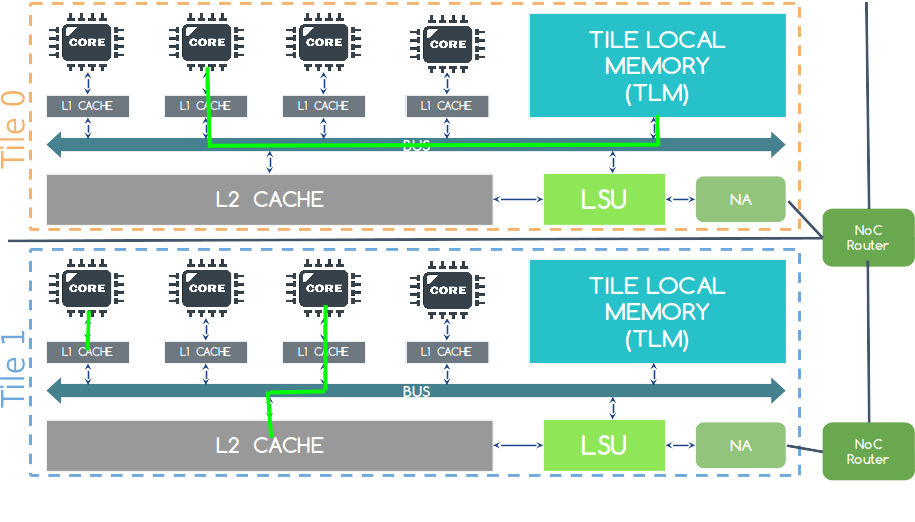
\includegraphics[width=\linewidth]{localaccesses.png}
  \centering
  \caption{A tile depicting local accesses to a TLM.}
  \label{fig:localaccesses}
\end{figure}
\subsubsection{Remote TLM Accesses}
Figure \ref{fig:remoteaccesses} depicts a scenario where a core is accessing another tiles TLM which makes it a remote TLM access. In this scenario the data transfer is happening over the bus and traffic is generated. Also, this takes more time since data is placed far away from the core that uses it. 
\begin{figure}
  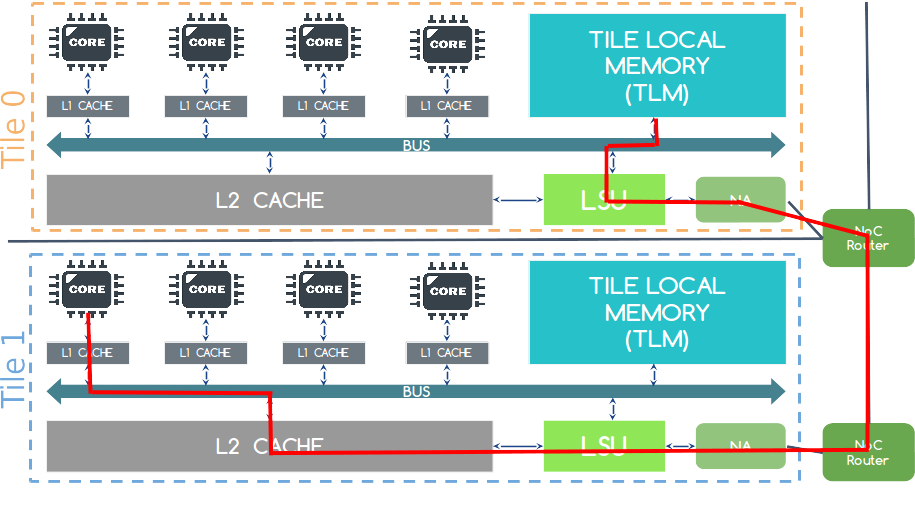
\includegraphics[width=\linewidth]{remoteaccesses.png}
  \centering
  \caption{A tile depicting remote accesses to a TLM.}
  \label{fig:remoteaccesses}
\end{figure}
\subsection{Goal}
We want to reduce the number of remote TLM accesses since it takes more time to fetch data from a TLM which is placed on another tile (as the request has to go on the bus through the network adapter and over the NoC Router in order to go to the other tile) and less time to fetch data which is on a core's own tile.  
\section{Modules Directly Used in the System for Implementing Thesis}
\subsection{Trace File}
As we use a trace based processor model, we first generate and save the traces using the gem5 simulator~\cite{gem5}. We build gem5 for Alpha ISI and use the modified Linux kernel and disk image from~\cite{trace} to execute benchmarks in full system mode~\cite{lispaper}.
\subsection{Memory Management Unit}
The Memory Management Unit (MMU) sits between the trace file and the core's as shown in Figure \ref{fig:traceFile}. This unit is basically a table which contains the address translation of all the addresses from the DRAM to the TLM. At start all TLM's are empty which means every instruction has to access data from the DRAM. The vector address table is updated if the DRAM is accessed or if migration is triggered by the Central Stats Module and if that migration takes place.
\subsection{Cache Stats Module}
The Cache Stats module is connected to the L1 and L2 Caches and is continuously getting updates from them regarding cache hits and misses per cache line. This module is responsible for calculating the cache hits and misses per TLM Block and to calculate for every TLM block the number of local and remote accesses. It also plays a important role in carrying out the data migration command as the migration command has to go through this module. 
\subsection{Tile Local Memory Module}
This is the Tile's Local Memory and has been explained in detail in chapter 2. This module also has the functionality to observe itself and calculate whether it is empty, is full or has free space. If it has free space then it can find the staring and ending address of all the free spaces. 
\subsection{Central Stats Module}
This is the main central module which all the Cache Stats modules and TLM Mem modules are reporting to. This module is responsible of finding whether migration shall take place or not and to send out invalidation commands for the data that has to be moved in case if migration has to be triggered. 
\section{System Design}
Figure~\ref{fig:overviewOfSolution} shows the overview of the modules involved in dynamic migration scheme. Every cache module is connected to a Cache Stats module. All these Cache Stats modules and the TLM MEM modules report to the Central Stats Module at every given time interval (T$_{interval}$). The Central Stats Module does evaluation of this data and triggers migration if needed. \\
\\
Also, there is a vector address table which sits between the trace file and the CPU's as shown in Figure \ref{fig:traceFile}. Every instruction from the trace file first passes through the vector address table for address translation and then it is executed.\\
\begin{figure}[h!]
  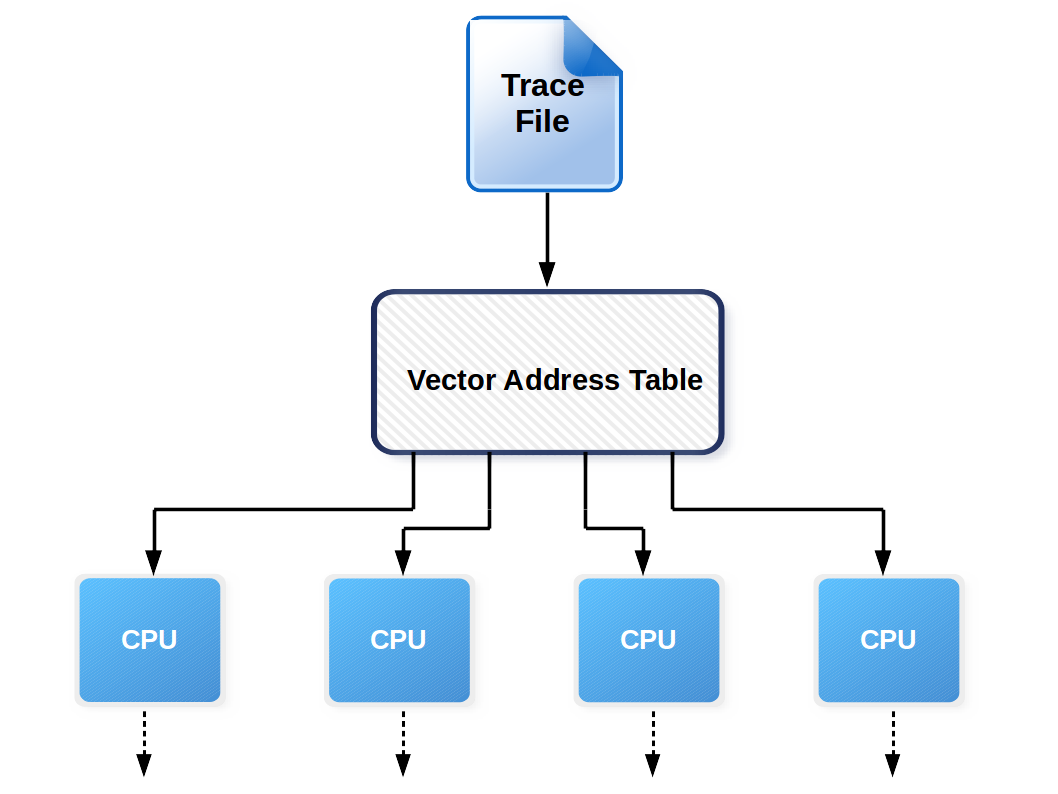
\includegraphics[width=0.7\linewidth]{traceFile.png}
  \centering
  \caption{Vector Address Table and Trace File Placement}
  \label{fig:traceFile}
\end{figure}
\begin{figure}
  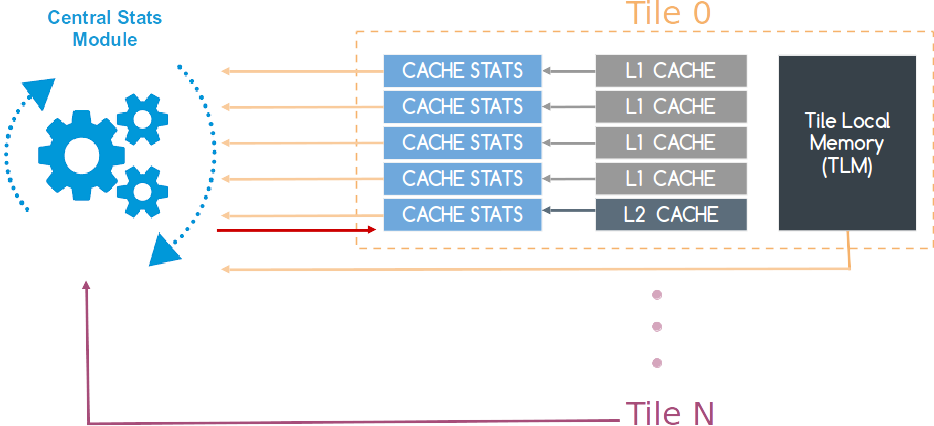
\includegraphics[width=\linewidth]{moduleconnections.png}
  \centering
  \caption{Figure illustrating the overview of the modules used.}
  \label{fig:overviewOfSolution}
\end{figure}
\\
Figure \ref{fig:approachOfSolution} shows the messages exchanged between the Cache Stats, TLM Mem and Central Stats Module. At every given time interval (T$_{interval}$) the Cache Stats module sends the number of local and remote accesses of all the TLM blocks to the Central Stats module and the TLM MEM module sends its free address space to the Central Stats module. The TLM block size is equal to a variable number of cache lines that is determined at compile time by the user. The Central Stats module then evaluates this received data and sends a migrate command to the L2 Cache Stats module if it thinks that migration is needed. \\
\\
The next subsections will explain how the messages exchanged between the modules are calculated. 
\begin{figure}
  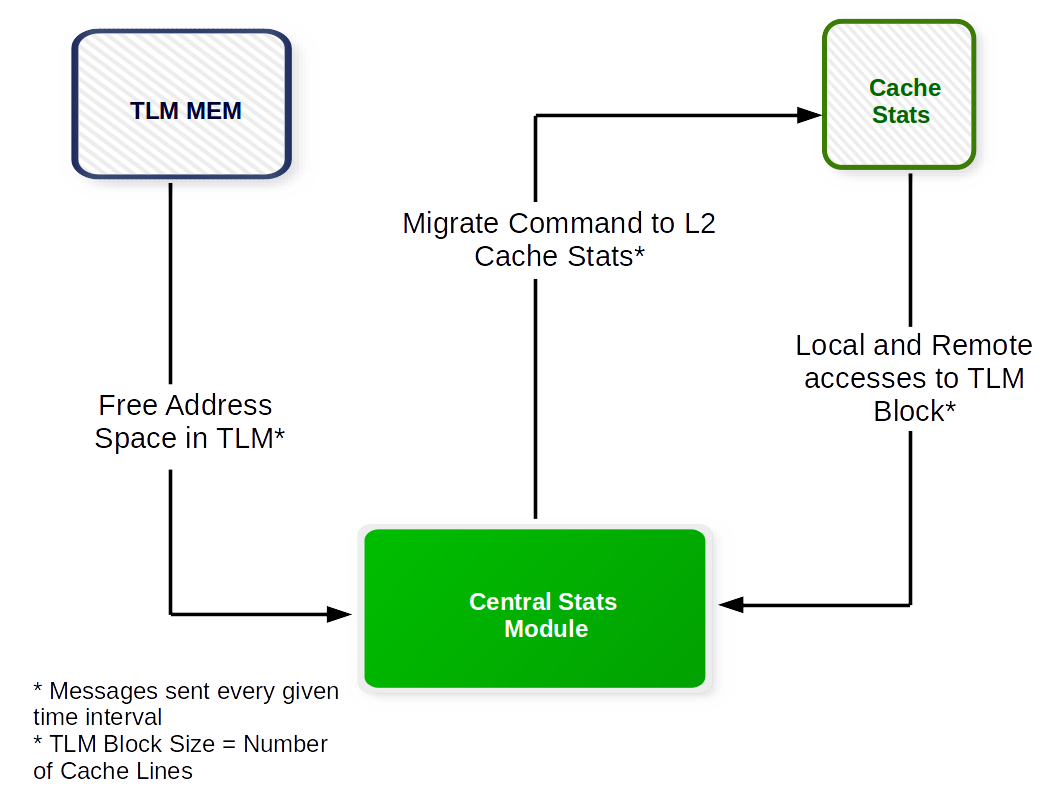
\includegraphics[width=0.8\linewidth]{approachOfSolution.png}
  \centering
  \caption{Messages exchanged between different modules.}
  \label{fig:approachOfSolution}
\end{figure}
\subsection{Local and Remote Accesses to a TLM Block}
Figure \ref{fig:remoteLocalAccess} shows the calculation behind the metric of local access and remote access to a TLM Block in the Cache Stats module. We compare the TLM number which is being accessed by a instruction with the current tile number (the tile where the cache stats module is placed). If the two values are equal it means it is a request to the TLM of the same tile which signifies it is a local access. If the two values are different it implies it is a request for another tile's TLM and we check whether there is a L1 cache hit or miss. If there is a L1 cache hit, it is a local access. However, if it is a L1 cache miss then we check whether it is a L2 cache hit or miss. If it is a hit then it a local access but if it is a miss then we have a remote access. \\
\begin{figure}
  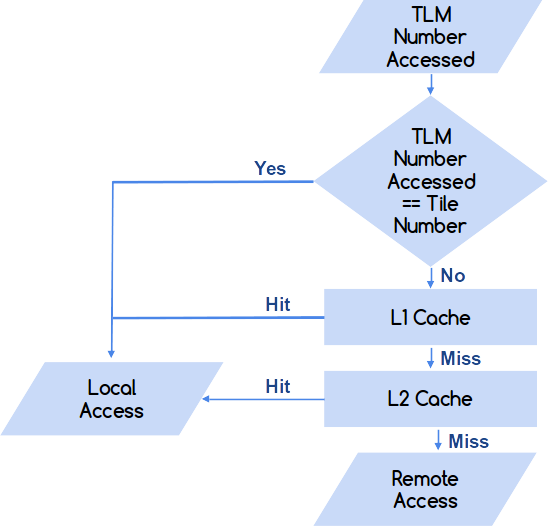
\includegraphics[width=0.6\linewidth]{localandremote.png}
  \centering
  \caption{Flowchart illustrating how to determine a local and remote TLM access.}
  \label{fig:remoteLocalAccess}
\end{figure}

\subsection{Free Address Space in TLM}
Figure \ref{fig:freeSpaceTLM} shows how we find the free address space in the TLM MEM module. For calculating the free address space in the TLM we can have three scenarios. 
\begin{figure}
  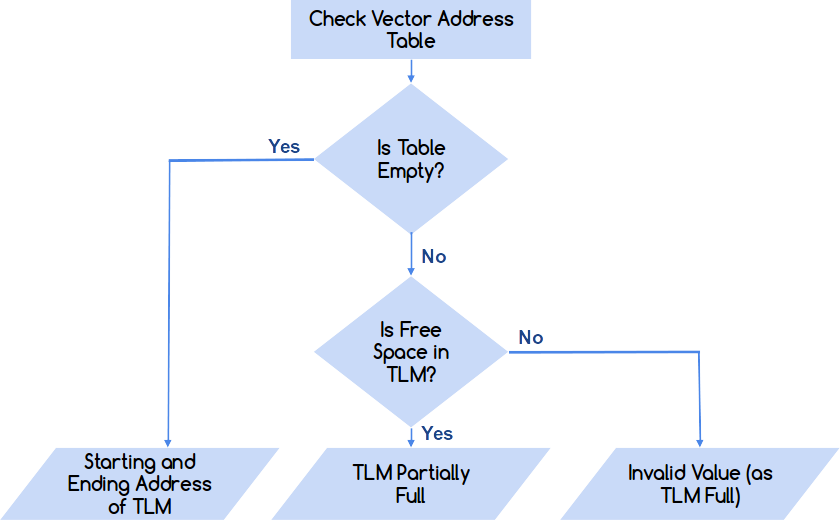
\includegraphics[width=\linewidth]{freespace.png}
  \centering
  \caption{Flowchart depicting how the free address space in the TLM is calculated.}
  \label{fig:freeSpaceTLM}
\end{figure}
\begin{enumerate}
  \item TLM Empty 
  \item TLM Partially Full
  \item TLM Full
\end{enumerate}
\subsubsection{TLM Empty}
If the vector address table is empty then we know straightaway that the TLM is empty. In that scenario, the starting and ending address of the TLM address space are sent to the Central Stats Module.\\ 
\subsubsection{TLM Partially Full}
If the vector address table is not empty we iterate over the table and extract the addresses belonging to the current tile's TLM. After we have these addresses we analyze them and determine the free address space in the TLM. The starting and ending address of one free space block is send to the Central Stats Module.\\
\begin{figure}
  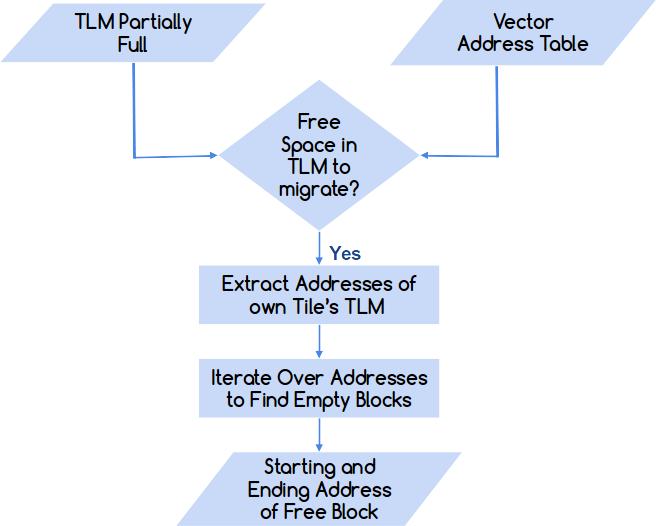
\includegraphics[width=0.7\linewidth]{tlmpartiallyempty.png}
  \centering
  \caption{Flowchart showing how the free address space in TLM is calculated if the TLM is partially full.}
  \label{fig:freeSpaceTLM}
\end{figure}
\subsubsection{TLM Full}
In this case also the vector address table is not empty. We extract the addresses belonging to the current tile's TLM and if there isno space in the TLM we inform the Central Stats Module this by sending a invalid value.\\
\subsection{Triggering Migrations}
\subsubsection{Which TLM Block to Migrate and Tile to Migrate it to?}
Figure \ref{fig:tiletomigrate} shows the the tile to migrate a certain TLM block is determined. In the Central Stats Module first it is determined whether a TLM Block shall be migrated or not and if it has to be migrated then it is decided which tile to migrate it to. This decision is based on the local and remote accesses to the specific TLM block (explained in detail above). For every TLM Block, the tile with the maximum remote accesses is found and if these remote accesses are greater than local accesses it means it has to be migrated to this tile.\\
\begin{figure}
  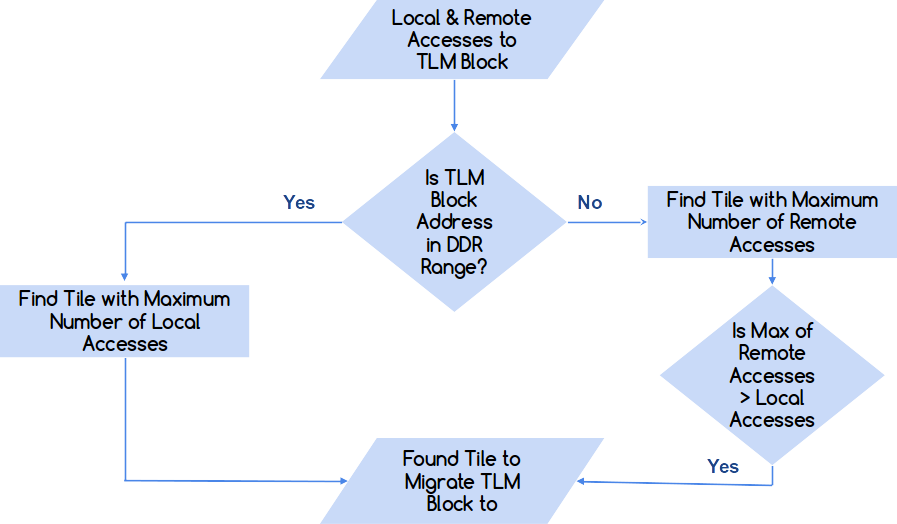
\includegraphics[width=0.4\linewidth]{tiletomigrate.png}
  \centering
  \caption{Process to determine the TLM Block to migrate and the tile to migrate the TLM Block to.}
  \label{fig:tiletomigrate}
\end{figure}
\subsubsection{When to Trigger Migrations?}
Figure \ref{fig:tlm_stats flowchart} shows the algorithm for determining when migration shall take place. After we know the tile to which a specific TLM Block shall me migrated, it is determined whether there is free space in that tile's TLM. If there is free space, a migration command is send to L2 Cache Stats module. \\
\\
However, if there is no free space in the TLM, then the block with the least number of local accesses in the TLM is identified and this number of local accesses is compared with the number of remote accesses of the TLM block which is to be migrated. If the number of remote accesses of the TLM block to be migrated is higher than this number of local accesses a migration command is send to the L2 Cache Stats module for this block in-order to migrate it to the DDR i.e this block is migrated back to the DDR and free space is made for the incoming TLM block. Now with free space in the TLM a migration command is send to the  L2 Cache Stats module for the TLM block to be migrated to the tile. If the remote accesses of the TLM block to be migrated are less than the minimum local accesses in the TLM then the migration is flushed.\\
\\
In case all the local accesses to a TLM are equal and a minimum cannot be found then at random a TLM Block is picked and the local accesses are compared with the migrating TLM Block's remote accesses. If the former is smaller than the latter, the TLM block is migrated to the DDR and free space is made for the incoming TLM block. Now with free space in the TLM a migration command is send to the  L2 Cache Stats module for the TLM block to be migrated to the tile. \\
\subsubsection{Migrate Command}
The migrate command is split into two commands in the Cache Stats module; first reading data from the location from where data has to be migrated and then writing data at the new location to which the migration is taking place. Once, the data is read a invalidation command is sent to all L1 and L2 caches for that TLM Block and once the data is written the vector address table is updated. \\
\begin{figure}
  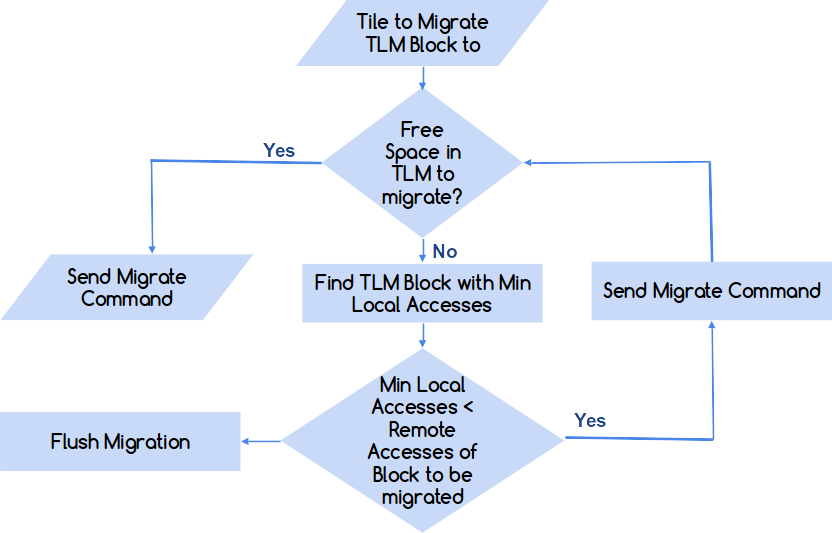
\includegraphics[width=\linewidth]{tlmstats.png}
  \centering
  \caption{Triggering Migration Commands}
  \label{fig:tlm_stats flowchart}
\end{figure}
\section{Usability Improvement}
In the simulator we have now given an option to turn dynamic data migration on and off by setting a parameter from the command line or from within the tool Synopsys. It makes the result gathering phase very easy. Also, since the TLM Block size and the time interval (T$_{interval}$) are variable and can be changed by the user; the change in performance or execution time by varying these two parameters can be analyzed.
\section{Limitations}
Adding the dynamic data migration support to the simulator increased the real time of the simulation by quite an extend. \\
\\
In the simulator the main modules added because of the dynamic data migration scheme are:
\begin{itemize}
  \item Twenty Cache Stats modules
  \item One Central Stats module 
  \item One Vector Address Table
\end{itemize}
The memory needed for these modules also add quite an overhead to the system. 
\begin{table}[h!]
\begin{center}
 \begin{tabular}{||c c c c||} 
 \hline
 Module & Size & Memory Usage   & Resource Utilization \\ [0.5 ex] 
 \hline\hline
 Cache Stats Module & xx & xxx & xxxx \\ 
 \hline
 Central Stats Module & xx & xxx & xxxx \\
 \hline
 Vector Address Table & xx & xxx & xxxx \\
 \hline\hline
 Total  & xx & xxx & xxxx \\
  \hline
\end{tabular}
 \caption{Table showing the size of the modules}
\end{center}
\end{table}
\\
\\
complexity of the algorithm
\chapter{Experimental Setup}
This chapter will lay out the programs that assisted in running the simulations. Moreover, it will also illustrate the specifications of the machine that were utilized to run the experiments.
\section{The gem5 Simulator and Trace Files}
The gem5 simulator~\cite{gem5} is a modular platform for computer system architecture research, encompassing system-level architecture as well as processor micro-architecture. We use the gem5 full system simulator to generate the trace file for the simulations. For all our simulations, we make use of workloads from the PARSEC Benchmark Suite~\cite{lispaper}. We choose four parallel workloads covering three application domains and generate their trace files:
\begin{itemize}
\item Blackscholes, Swaptions (Financial Analysis)
\item Canneal (Engineering)
\item Fluidanimate (Animation)
\end{itemize}
\section{Platform Architect MCO}
The simulator is designed in Synopsys Platform Architect MCO~\cite{synopsys}. It gives a graphical environment for configuring and analyzing the system. 
\section{Writing Shell Script}
A shell script for running the migration command is written so that multiple simulations can run in parallel without the need to recompile the simulator. The maximum number of parallel simulations that we could run was four. This saved us considerable time in gathering results. 
\section{\textit{Nice} Command}
The script is run with \textit{nice} command~\cite{nice} which runs the simulation with a different priority then the usual. We ran the simulations with a increased priority of nine.
\section{Output Files}
The output of the simulation is saved in different text files. The files important for this thesis are:
\begin{itemize}
\item Screen Log File
\item Time Log File
\end{itemize}
\subsection{Screen Log File}
The screen log file gives the virtual processing time (in nano seconds) of each processor and also of the entire system. It also gives the real time, the user time and the system time of running the simulations in minutes and seconds. Further it gives the total number of remote reads and remote writes of the simulation run and some other parameters and queue sizes that are not relevant for this thesis.\\
\subsection{Time Log File}
The time log file consists of the breakdown of the virtual time (in nano seconds) that each processor took executing instructions on different tiles and on the individual components/modules like TLM, L1-Cache, NPC, NoC, Bus etc.
\section{System Specifications}
The simulations were run on a core i5 Intel processor with a Solid-State-Drive (SSD) ---? in-order to reduce the real time for the simulations. Ubuntu..
\chapter{Evaluation}

\chapter{Conclusion and Outlook}


% --- Bibliography
\cleardoublepage
\bibliographystyle{plain}
\bibliography{thesis}

% --- Mandatory confirmation.
\confirmation

\end{document}

%%% Local Variables:
%%% mode: latex
%%% TeX-master: t
%%% End:
